\begin{figure}[htp]
\centering
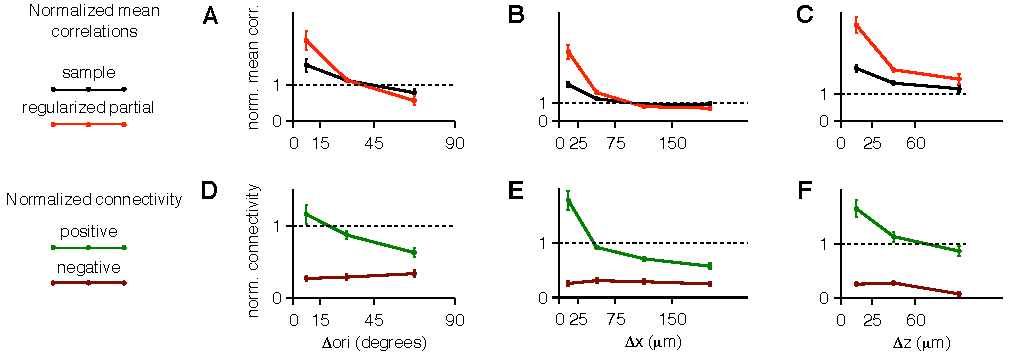
\includegraphics[width=0.5\textwidth]{figures/Figure6.pdf}
\caption{
Relationship between the structure of the estimate and the functional and spatial organization of the circuit.
{\bf A:} Average sample correlation, average partial sample correlation, and average partial correlation in the sparse+low-rank estimate for site in Fig.~\ref{fig:05} as a function of difference in cortical depth within the same column.
{\bf C:} Average sample correlation, average partial sample correlation, and average partial correlation in the sparse+low-rank estimate for site in Fig.~\ref{fig:05} as a function of lateral distance at the same cortical depth.
{\bf E,G:} Average sample correlation, and interaction probability obtained from the sparse+low-rank estimate as well as by thresholding the sample correlation matrix to equal sparsity as function of difference in cortical depnth and lateral distance.
{\bf I:} Average sample correlation, and interaction probability obtained from the sparse+low-rank estimate as well as by thresholding the sample correlation matrix to equal sparsity as a function of difference in preffered orientation.
}
\label{fig:06}
\end{figure}
